

\begin{frame}{\ft{3D Graphics Sent to MeshLab}}
\section{Research Slide 2}

\doubleFrame{... Once the 3D tissue sample is constructed by 3DimViewer's algorithms, 
an \AtR{} inter-application networking protocol (implemented 
as an extension to both applications) allows 3DimViewer to 
export the model to MeshLab so that it may be studied in a 
more comprehensive 3D viewing environment.}

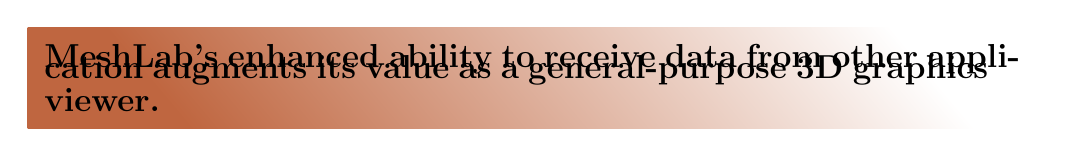
\begin{tikzpicture}
\nodeincludegraphicsTR{2.7cm}{2cm}{pics/RAD-3.png}

% \node [anchor=west,fill=brown!20!white,inner sep=7, text width=14cm]
%  (longnote) at (5.5,7) {%  %{\color{rb!85!red}{
%  {\cframedbox{\large \textbf{EC3}}}};

 \node [anchor=west,bottom color=brown!80!purple,
 top color=white, %top color=blue!40!cyan, 
 shading angle=310, 
 inner sep=6, text width=12.6cm]
  (longnote) at (10.5,15.4) {\vspace{-8pt}%  %{\color{rb!85!red}{
  {\cframedboxblue{\large \textbf{MeshLab's 
enhanced ability to receive data from other application 
augments its value as a general-purpose 3D graphics viewer.}}}};

\end{tikzpicture}


\end{frame}

